
\subsection{Statischer Verstärkungsfaktor}

Der statischer Verstärkungsfaktor des behandelten $IT_1-Gliedes$ beträgt: \[K=4\]
Ein Graph des Verstärkungsfaktor, wobei auf der $x-Achse$ die konstanten Eingänge und auf der $y-Achse$ die Ausgänge des Systems für $t \rightarrow \infty$ aufgetragen sind, ist in Abbildung~\ref{fig:static-curve} zu sehen. \\

\begin{figure}[H]
	\centering
	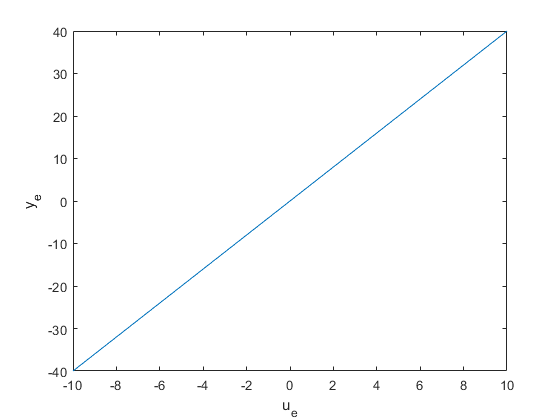
\includegraphics[width=0.7\linewidth]{{diagrams/staticCurve.png}}
	\caption[Statische Verstärkung]{Statische Verstärkung}
	\label{fig:static-curve}
\end{figure}